\documentclass{beamer}
%
% Choose how your presentation looks.
%
% For more themes, color themes and font themes, see:
% http://deic.uab.es/~iblanes/beamer_gallery/index_by_theme.html
%
\mode<presentation>
{
  \usetheme{Boadilla}      % or try Darmstadt, Madrid, Warsaw, ...
  \usecolortheme{beaver} % or try albatross, beaver, crane, ...
  \usefonttheme{default}  % or try serif, structurebold, ...
  \setbeamertemplate{navigation symbols}{}
  \setbeamertemplate{caption}[numbered]
  
} 

\usepackage{xcolor,colortbl}
\usepackage[english]{babel}
\usepackage[utf8x]{inputenc}
\usepackage{courier}
\usepackage{dsfont}
\usepackage{verbatim} 
\usepackage{enumerate}
\usepackage{tikz}
\usepackage{multirow}
\usepackage{bbm}
\usepackage{amsmath}
\usepackage{venndiagram}
\usepackage{epigraph} 
%\usepackage{xcolor}



\usepackage{hyperref}
\hypersetup{
    colorlinks=true,
    linkcolor=blue,
    filecolor=magenta,      
    urlcolor=cyan,
}

% R stuff!
\usepackage{listings}
\definecolor{codegreen}{rgb}{0,0.6,0}
\definecolor{codegray}{rgb}{0.5,0.5,0.5}
\definecolor{codepurple}{rgb}{0.58,0,0.82}
\definecolor{backcolour}{rgb}{0.95,0.95,0.92}

\lstdefinestyle{mystyle}{
    backgroundcolor=\color{backcolour},    
    commentstyle=\color{codegreen},
    keywordstyle=\color{black},
    numberstyle=\tiny\color{codegray},
    stringstyle=\color{codepurple},
    basicstyle=\ttfamily\footnotesize,
    breakatwhitespace=false,         
    breaklines=true,                 
    captionpos=b,                    
    keepspaces=true,                 
    numbers=left,                    
    numbersep=5pt,                  
    showspaces=false,                
    showstringspaces=false,
    showtabs=false,                  
    tabsize=2
}

\lstset{style=mystyle}



%% Size options for nested itemized lists
\usepackage{relsize}
\setbeamerfont{itemize/enumerate body}{parent=normal text}
\setbeamerfont{itemize/enumerate subbody}{parent=normal text,size=\relsize{-1}}
%\setbeamerfont{itemize/enumerate subsubbody}{parent=normal text,size=\relsize{-1}}




\setbeamertemplate{enumerate items}[default]
\setbeamertemplate{itemize item}[triangle]

%\setitemize{label=\usebeamerfont*{itemize item}%
%  \usebeamercolor[fg]{itemize item}
%  \usebeamertemplate{itemize item}}


\usetikzlibrary{shapes,decorations,arrows,calc,arrows.meta,fit,positioning}
\tikzset{
    -Latex,auto,node distance =1 cm and 1 cm,semithick,
    state/.style ={ellipse, draw, minimum width = 0.7 cm},
    point/.style = {circle, draw, inner sep=0.04cm,fill,node contents={}},
    bidirected/.style={Latex-Latex,dashed},
    el/.style = {inner sep=2pt, align=left, sloped}
}

\newcommand{\Mypm}{\mathbin{\tikz [x=1.4ex,y=1.4ex,line width=.1ex] \draw (0.0,0) -- (1.0,0) (0.5,0.08) -- (0.5,0.92) (0.0,0.5) -- (1.0,0.5);}}%



%% For block quote
\usepackage{etoolbox}
\AtBeginEnvironment{quote}{\par\singlespacing\small}


\title[STA-209]{Inference for Multivariate Regression}
\subtitle{ANOVA for MLR}
%\author{}
\author{Grinnell College}
\date{December 9, 2024}

\graphicspath{{img/}}

\begin{document}

\begin{frame}
  \titlepage
\end{frame}

\begin{frame}{Review}

\begin{itemize}
\item Regression models a linear relationship between response variable $y$ and explanatory variable $X$ of the form
\begin{align*}
y = \beta_0 + \beta_1 X + \epsilon
\end{align*}
\item We can expand this to include \textit{combinations} of explanatory variables
\item in fact we saw this earlier on in the semester too, albeit briefly
\end{itemize}

\end{frame}


\begin{frame}{Cases}

\begin{columns}

  \begin{column}{0.4\textwidth}
\begin{enumerate}
\item $y = \beta_0 + X \beta_1$ \vspace{4mm}
\item $y = \beta_0 + \mathbbm{1}_A \beta_1 $ \vspace{4mm}
\item $y = \beta_0 + \mathbbm{1}_A \beta_1 + X \beta_2 $ \vspace{4mm}
\item $y = \beta_0 + \mathbbm{1}_A \beta_1 + \mathbbm{1}_B \beta_2 $ \vspace{4mm}
\item $y = \beta_0 + X_1 \beta_1 + X_2 \beta_2 $ \vspace{4mm}
\end{enumerate}
  \end{column}
  \begin{column}{0.5\textwidth}
\begin{enumerate}
\item Simple linear, $\beta_1$ shows change in  $y$ given change in $X$
\item Simple categorical, reference variable and group means
\item Continuous and categorical, two regression lines with same slope but different intercept
\item Multiple categorical, combined reference variables
\item Multiple continuous, $\beta_1$ shows change in $y$ given change in $X_1$, \textit{assuming everything else held constant}
\end{enumerate}
  \end{column}

\end{columns}
\end{frame}


\begin{frame}[fragile]{Single Quantiative}

\begin{lstlisting}[language=R]
> lm(mpg ~ wt, mtcars) %>% summary()


Coefficients:
            Estimate Std. Error t value        Pr(>|t|)    
(Intercept)   37.285      1.878   19.86 < 0.00000000002 ***
wt            -5.344      0.559   -9.56        0.000013 ***


Residual standard error: 3.05 on 30 degrees of freedom
Multiple R-squared:  0.753,	Adjusted R-squared:  0.745 
F-statistic: 91.4 on 1 and 30 DF,  p-value: 0.000000000129
\end{lstlisting}

\end{frame}

\begin{frame}{Weight and MPG}
\begin{align*}
\hat{y} = 37.285 - 5.34 \times \text{Weight}
\end{align*}
\begin{center}
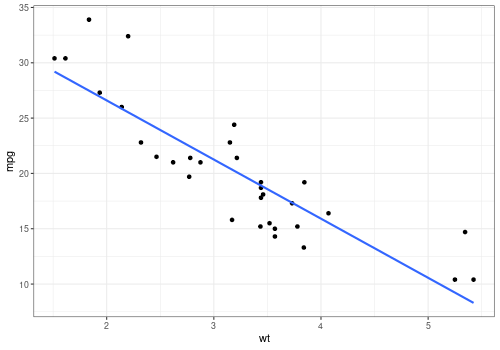
\includegraphics[scale=0.5]{wt_mpg.png}
\end{center}
\end{frame}


\begin{frame}[fragile]{Single Categorical}

\begin{lstlisting}[language=R]
> lm(mpg ~ cyl, mtcars) %>% summary()

Coefficients:
            Estimate Std. Error t value        Pr(>|t|)    
(Intercept)   26.664      0.972   27.44 < 0.00000000002 ***
cyl6          -6.921      1.558   -4.44         0.00012 ***
cyl8         -11.564      1.299   -8.90   0.00000000086 ***


Residual standard error: 3.22 on 29 degrees of freedom
Multiple R-squared:  0.732,	Adjusted R-squared:  0.714 
F-statistic: 39.7 on 2 and 29 DF,  p-value: 0.00000000498
\end{lstlisting}

\end{frame}

\begin{frame}{Cylinder and MPG}
\begin{align*}
\hat{y} = 26.66 - 6.92 \times \mathbbm{1}_{6 \text{cyl}} - 11.564 \times \mathbbm{1}_{8 \text{cyl}}
\end{align*}
\begin{center}
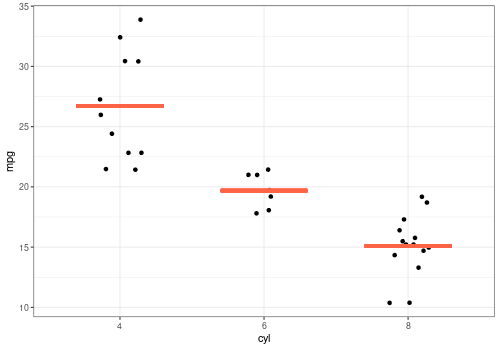
\includegraphics[scale=0.5]{cyl_mpg.png}
\end{center}
\end{frame}

\begin{frame}[fragile]{Categorical and Quantitative}

\begin{lstlisting}[language=R]
> lm(mpg ~ wt + cyl, mtcars) %>% summary()

Coefficients:
            Estimate Std. Error t value        Pr(>|t|)    
(Intercept)   33.991      1.888   18.01 < 0.00000000002 ***
wt            -3.206      0.754   -4.25         0.00021 ***
cyl6          -4.256      1.386   -3.07         0.00472 ** 
cyl8          -6.071      1.652   -3.67         0.00100 ***


Residual standard error: 2.56 on 28 degrees of freedom
Multiple R-squared:  0.837,	Adjusted R-squared:  0.82 
F-statistic: 48.1 on 3 and 28 DF,  p-value: 0.0000000000359
\end{lstlisting}

\end{frame}

\begin{frame}{Cylinder, weight and MPG}
\begin{align*}
\hat{y} = 33.99 - 3.21 \times \text{weight} - 4.26 \times \mathbbm{1}_{6 \text{cyl}} - 6.07 \times \mathbbm{1}_{8 \text{cyl}}
\end{align*}
\begin{center}
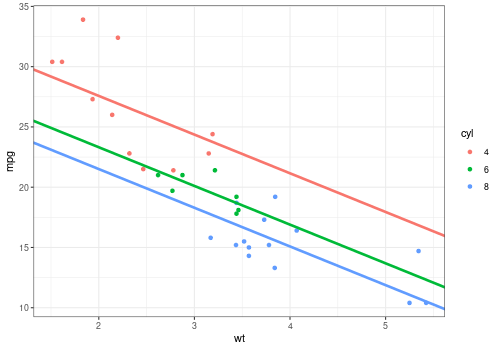
\includegraphics[scale=0.5]{cyl_wt_mpg.png}
\end{center}
\end{frame}



\begin{frame}[fragile]{Multiple Categorical}

\begin{lstlisting}[language=R]
> lm(mpg ~ cyl + am, mtcars) %>% summary()

Coefficients:
            Estimate Std. Error t value        Pr(>|t|)    
(Intercept)    24.80       1.32   18.75 < 0.00000000002 ***
cyl6           -6.16       1.54   -4.01         0.00041 ***
cyl8          -10.07       1.45   -6.93      0.00000015 ***
am1             2.56       1.30    1.97         0.05846 .  


Residual standard error: 3.07 on 28 degrees of freedom
Multiple R-squared:  0.765,	Adjusted R-squared:  0.74 
F-statistic: 30.4 on 3 and 28 DF,  p-value: 0.00000000596
\end{lstlisting}

\end{frame}

\begin{frame}{Cylinder, transmission and MPG}
\begin{align*}
\hat{y} = 24.8  - 6.16 \times \mathbbm{1}_{6 \text{cyl}} - 10.07 \times \mathbbm{1}_{8 \text{cyl}} + 2.56 \times \mathbbm{1}_{Manual}
\end{align*}
\begin{center}
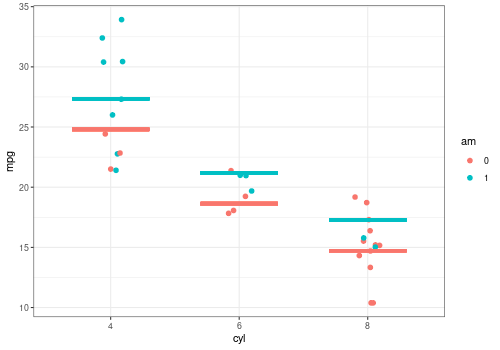
\includegraphics[scale=0.5]{cyl_am_mpg.png}
\end{center}
\end{frame}


\begin{frame}[fragile]{Multiple Quantitative}

\begin{lstlisting}[language=R]
> lm(mpg ~ wt + disp, mtcars) %>% summary()

Coefficients:
            Estimate Std. Error t value         Pr(>|t|)    
(Intercept) 34.96055    2.16454   16.15  0.000000049 ***
wt          -3.35083    1.16413   -2.8        0.0074 ** 
disp        -0.01772    0.00919   -1.93       0.0636 .  


Residual standard error: 2.92 on 29 degrees of freedom
Multiple R-squared:  0.781,	Adjusted R-squared:  0.766 
F-statistic: 51.7 on 2 and 29 DF,  p-value: 0.000000000274
\end{lstlisting}

\end{frame}

\begin{frame}{Cylinder, transmission and MPG}
\begin{align*}
\hat{y} = 34.96 - 3.35 \times \text{weight} - 0.017 \times \text{displacement}
\end{align*}
\begin{center}
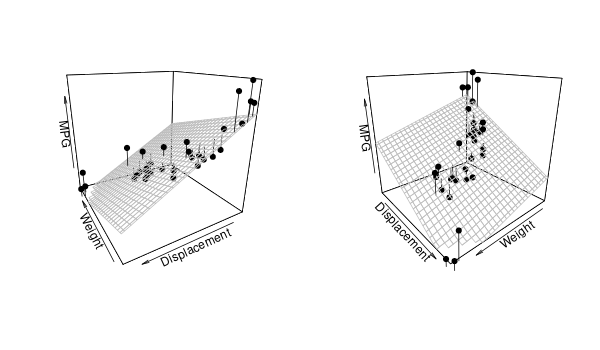
\includegraphics[scale=0.5]{wt_disp_mpg.png}
\end{center}
\end{frame}




\begin{frame}[fragile]{Multiple Quantiative and categorical}
\footnotesize

\begin{lstlisting}[language=R]
> lm(mpg ~ wt + disp + am,  mtcars) %>% summary()

Coefficients:
            Estimate Std. Error t value       Pr(>|t|)    
(Intercept) 34.67591    3.24061   10.70 0.000000000021 ***
wt          -3.27904    1.32751   -2.47          0.020 *  
disp        -0.01780    0.00937   -1.90          0.068 .  
am1          0.17772    1.48432    0.12          0.906    


Residual standard error: 2.97 on 28 degrees of freedom
Multiple R-squared:  0.781,	Adjusted R-squared:  0.758 
F-statistic: 33.3 on 3 and 28 DF,  p-value: 0.00000000225
\end{lstlisting}


\end{frame}


\begin{frame}{Multiple quantiative with categorical}
\begin{align*}
\hat{y} = 34.67 - 3.27 \times \text{weight} - 0.018 \times \text{displacement} + 0.17 \times \mathbbm{1}_{Manual}
\end{align*}
\begin{center}
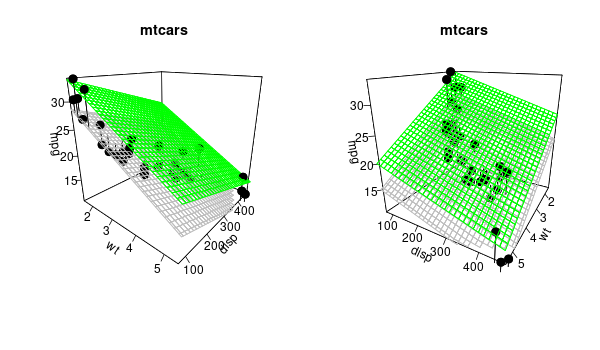
\includegraphics[scale=0.5]{wt_disp_am1.png}
\end{center}
\end{frame}

\begin{frame}{Correlated Explanatory Variables}
We have been using the fact that there is correlation between the response and explanatory variables
\begin{itemize}
    \item correlation coefficient (r) measured this for SLR
    \item larger $|r|$ value $\rightarrow$ larger correlation $\rightarrow$ better predictions
\end{itemize} \vspace{10mm}

It actually turns out there can be correlation between the explanatory variables too
\begin{itemize}
    \item this is actually \textit{not} good (bad)
    \item intuition: if there is correlation between explanatory variables then each explanatory variable tells us info about the other
    \item this actually means we are effectively using \textit{less} than 2 explanatory variables because the variables have overlapping info about response $y$
\end{itemize}
\end{frame}


\begin{frame}[fragile]{Correlated Explanatory Variables}
\footnotesize

Regression: predicting MPG with Weight
\begin{lstlisting}[language=R]
> lm(mpg ~ wt, mtcars) %>% summary()


Coefficients:
            Estimate Std. Error t value     Pr(>|t|)    
(Intercept)   37.285      1.878   19.86   < 0.000002 ***
wt            -5.344      0.559   -9.56     0.000013 ***
\end{lstlisting} \vspace{2mm}

Regression: predicting MPG with Weight and Displacement
\begin{lstlisting}[language=R]
> lm(mpg ~ wt + disp, mtcars) %>% summary()

Coefficients:
            Estimate Std. Error t value      Pr(>|t|)    
(Intercept) 34.96055    2.16454   16.15  0.000000049 ***
wt          -3.35083    1.16413   -2.8        0.0074 ** 
disp        -0.01772    0.00919   -1.93       0.0636 .

> cor(mtcars$wt, mtcars$disp)
0.8879799
\end{lstlisting}

\end{frame}

\begin{frame}{Correlated Explanatory Variables}
\begin{center}
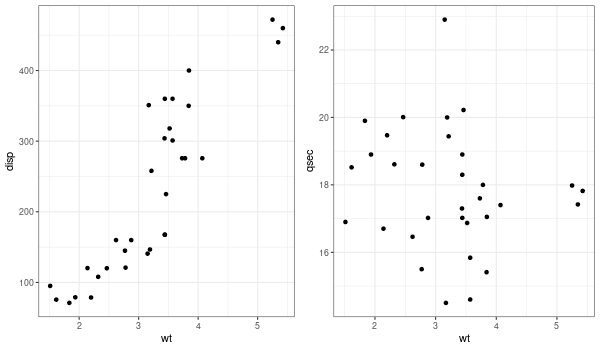
\includegraphics[scale=0.5]{cor_compare.png}
\end{center}
\end{frame}


\begin{frame}[fragile]{Correlated Explanatory Variables}


\begin{lstlisting}[language=R,basicstyle=\ttfamily\scriptsize]
> lm(mpg ~ wt, mtcars) %>% summary()

            Estimate Std. Error t value     Pr(>|t|)    
(Intercept)   37.285      1.878   19.86   < 0.000002 ***
wt            -5.344      0.559   -9.56     0.000013 ***
R-squared = 0.75

> lm(mpg ~ wt + disp, mtcars) %>% summary()

            Estimate Std. Error t value      Pr(>|t|)    
(Intercept) 34.96055    2.16454   16.15  0.000000049 ***
wt          -3.35083    1.16413   -2.8        0.0074 ** 
disp        -0.01772    0.00919   -1.93       0.0636 .  
R-squared = 0.78

> lm(mpg ~ wt + qsec, mtcars) %>% summary()

            Estimate Std. Error t value       Pr(>|t|)    
(Intercept)   19.746      5.252    3.76        0.00077 ***
wt            -5.048      0.484  -10.43 0.000000000025 ***
qsec           0.929      0.265    3.51        0.00150 ** 
R-squared = 0.82
\end{lstlisting}

\end{frame}




\begin{frame}{Key Takeaways}
\begin{itemize}
\item Quantitative variables represent slopes (changes in $X$ lead to $\beta$ changes in $y$)
\item Categorical variables represent horizontal shifts
\item Any number of categorical or quantiative variables can be added to model
\item Always interpret regression coefficients as \textit{everything else being fixed}
\item Look out for correlated variables
\begin{itemize}
    \item makes models harder to interpret and usually don't improve prediction much
\end{itemize}
\end{itemize}
\end{frame}

%\begin{frame}
%\begin{columns}
%
%  \begin{column}{0.45\textwidth}
%%
%  \end{column}
%  \begin{column}{0.45\textwidth}
%%
%  \end{column}
%
%\end{columns}
%\end{frame}


\end{document}